

\begin{refsection}
\chapter{Introduction} % Main chapter title

\label{Chapter1} % Change X to a consecutive number; for referencing this chapter elsewhere, use \ref{ChapterX}

%thispagestyle{empty}

%----------------------------------------------------------------------------------------
%	SECTION 1
%----------------------------------------------------------------------------------------

\section{Introduction}

\begin{sloppypar} The transcriptional and molecular machineries that control heart development are tremendously complex and sensitive to genetic and environmental disturbances. This is reflected by the high incidence of congenital cardiac anomalies in the human population, affecting approximately 1\% of all live births \cite{hoffman2002incidence}. Consequently, our insight into the etiology of heart malformations is directly linked to our understanding of cardiac development. \end{sloppypar}

Complex morphogenetic processes underlie the transformation of the tubular heart into four cardiac chambers with corresponding cardiac valves, venous inlets and arterial outlets (\cref{fig:1_1}). Aberrant development of any of the different cardiac components can potentially result in a congenital heart defect (CHD), which is defined as gross structural abnormality of the heart or intrathoracic great vessels that is actually or potentially of functional significance \cite{mitchell1971congenital}.

\begin{figure}[!tb]
\centering
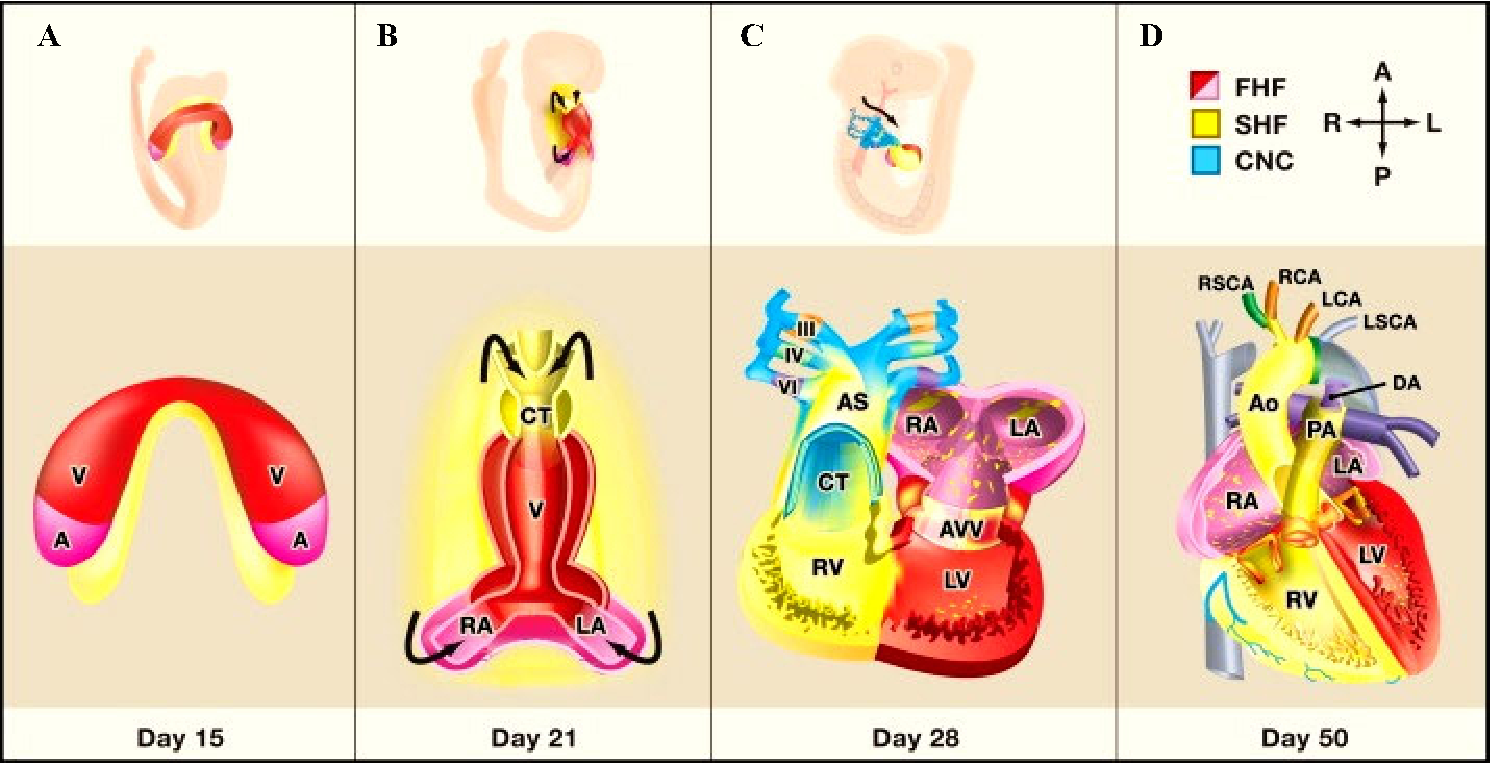
\includegraphics[scale=0.5,keepaspectratio]{Figures/Figure1_1.pdf}
\rule{35em}{0.5pt}
\caption[Developmental origin of cardiac structures]{\textbf{Developmental origin of cardiac structures:} Oblique views of whole embryos and frontal views of cardiac precursors during human cardiac development are shown. \textbf{A.} FHF cells form a crescent shape in the anterior embryo with SHF cells medial and anterior to the FHF, \textbf{B.} SHF cells begin to migrate (arrows) into the anterior and posterior ends of the tube to form the right ventricle, conotruncus, and part of the atria, \textbf{C.} Following rightward looping of the heart tube, cardiac neural crest cells also migrate (arrow) into the outflow tract from the neural folds to septate the outflow tract and pattern the bilaterally symmetric aortic arch arteries, \textbf{D.} Septation of the ventricles, atria, and atrioventricular valves results in the four-chambered heart. 
 A-artery, V-ventricle, CT- conotruncus, RV-right ventricle, LV-left ventricle, RA-right atrium, LA-left atrium, PA-pulmonary artery, Ao-aorta, Da-ductus arteriosus, RSCA, right subclavian artery, RCC-right common carotid, LCC-left common carotid, LSCA-left subclavian, AVV-atrioventricular valve. Source: \cite{srivastava2006genetic}}
\label{fig:1_1}
\end{figure}

Cardiogenesis is initiated with the formation of mesodermal multipotent cardiac progenitor cells, and is governed by cross‐talk between developmental cues emanating from both endodermal and ectodermal cells. The cells that form the embryonic ventricle of the heart are the first cardiac precursors to differentiate, and are thus collectively referred to as the first heart field (FHF). A large number of cardiac progenitor cells remain present as an undifferentiated sub-population medially and caudally to the cardiac crescent and tubular heart, and maintain their proliferative capacity before being added to the heart. These cardiac precursors are added after the formation of the tubular heart, and therefore have been dubbed the second heart field (SHF). Retrospective clonal analysis in the early developing mouse heart as well as several mouse studies have revealed that the onset of differentiation correlates with the addition of cells to the heart. These findings have led to the current paradigm that the heart tube elongates by recruitment of SHF cells that give rise to the outflow tract, right ventricle, the ventricular septum and to the remaining part of the left ventricle and the atria. Taken together, the FHF represents the cardiac precursors of the primitive myocardial crescent or bowl, and is important for the developing primitive ventricle of the tubular heart, whereas the remainder of the heart requires the ongoing contribution of SHF cells.

\section{Classification of CHD}

Heart defects are anatomically, clinically, epidemiologically, and developmentally heterogeneous. Classification for the purpose of etiological studies is both necessary and challenging. Basing classification on clinical type alone can lead to so many groups that specific genetic associations may be obscured. Ideally, an approach based on underlying developmental mechanisms can provide a rational basis for aggregating cases and preserve internal homogeneity Botto et al \cite{botto2007seeking} implemented an individual case classification method in which there is first identification of detailed cardiac malformations and then grouping based on similarity, complexity, and suspected embryologic origin. In their classification there are eight major groupings of human heart malformations. These are: (i) conotruncal, (ii) atrioventricular septal defects (AVSD), (iii) anomalous pulmonary venous return (APVR), (iv) left ventricular outflow tract obstruction (LVOTO), (v) right ventricular outflow tract obstruction (RVOTO), (vi) septal, (vii) heterotaxy, (viii) complex. Of the eight groups, conotruncal malformations arise from the impaired development of the SHF and account for approximately one third of all CHD.

\section{Conotruncal heart defects (CTHD)}

The conotruncal region of the developing heart refers to the area of the development and eventual location of the aortic and pulmonary valves, as well as the conal or outlet septum portion of the ventricular septum that lies in the plane between the two valves. CTHD result from either an error in septation, rotation, or a misalignment of their union and account for 25-30\% of all apparently isolated CHD \cite{srivastava2006genetic}.
The classic CTHD share the morphological architecture of the presence of ventricular outflow tract anomalies with normally related great arteries and involve cardiac structures that are, in part, derived from common cell lineages i.e. cardiac neural crest cells and the SHF. The common defects that have their origins in failure of development of the common outflow include tetralogy of fallot (TOF), pulmonary atresia with ventricular septal defect (PA-VSD), double outlet of right ventricular (DORV), transposition of the great arteries (TGA), persistent truncus arteriosus (TA) and interrupted aortic arch (IAA). The proportion of each subtype of CTHD remains more or less the same worldwide and is represented in \cref{fig:1_2}.


\begin{figure}[!tb]
\centering
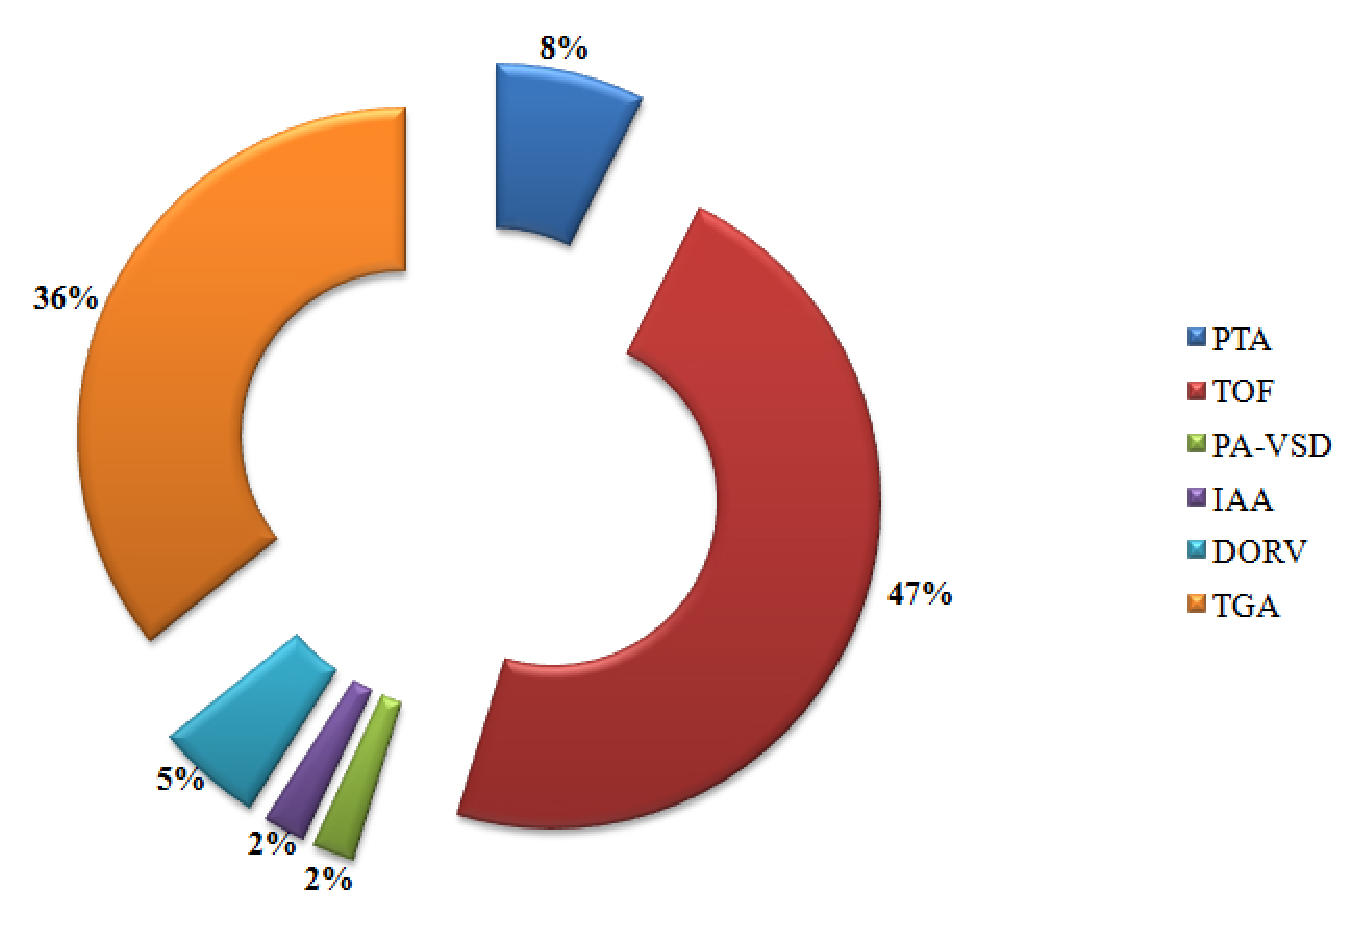
\includegraphics[scale=0.5,keepaspectratio]{Figures/Figure1_2.pdf}
\rule{35em}{0.5pt}
\caption[The proportion of different types of CTHD]{The proportion of different types of CTHD. \cite{pierpont2007genetic}}
\label{fig:1_2}
\end{figure}

\subsection{TOF} This is one of the most common forms of CTHD that causes cyanosis and is comprised of four separate components namely (i)ventricular septal defect (VSD), (ii)pulmonary stenosis (PS), (iii) ventricular hypertrophy and (iv) an overriding aorta .The VSD is usually large and blood flows from the RV through this into the LV. This occurs because of the resistance of blood flow through the pulmonary valve. Once the blood flows into the left ventricle, it is ejected into the aorta and delivers de-oxygenated blood into the body. Because there is de-oxygenated blood being delivered to the body, these babies may appear cyanotic, or "blue". Open heart surgery is needed to correct this defect. TOF occurs equally in boys and in girls.

\subsection{TGA} In this CTHD, the aorta originates from the RV and the PA from the LV. Because of this reversal, the aorta carries low-oxygen blood from the right ventricle to the body. The pulmonary artery carries oxygen-rich blood back to the lungs. In order for the infant born to survive, they must have some communication between the right and the left sides of the heart to allow-oxygen-rich blood to reach the body. This mixing of blood is possible through an ASD, VSD or PDA. Even though there is mixing of oxygenated and de-oxygenated blood, it is often not adequate to sustain life for an extended period of time. Babies with transposition are extremely blue at birth. The most common surgical procedure to correct this defect is called an arterial switch operation. Where the aorta is connected to the LV and the PA is connected to the RV. The ASD, VSD and/or PDA may also be needed to be corrected to restore normal blood flow. Sixty to seventy percent of the infants born with the defect are boys.

\subsection{PTA} In this defect, only one artery originates from the heart and forms both the aorta and the pulmonary artery. The truncus arises above a VSD that is almost always associated with this defect. The truncus receives low-oxygen blood from the right ventricle and oxygen-rich blood from the left ventricle. This mix of high and low-oxygen blood is sent out to the body and to the lungs. Open heart surgery in infancy is needed to correct this defect. The surgery involves closure of the VSD and removal of the pulmonary arteries from the truncus. The pulmonary arteries are then connected to the RV with a prosthetic tube which usually needs to be replaced as the infant grows.

\subsection{DORV} Normally, a ventricle has just one outlet which for the LV is the aorta and for the right ventricle is the PA. However, in DORV, both of these outlet blood vessels arise from the RV, either totally or to a great extent. Most cases of DORV have a VSD.

\subsection{PA/VSD} This is a cyanotic congenital heart disease characterized by underdevelopment of the RV outflow tract with atresia of the pulmonary valve, a large VSD and overriding of the aorta. In this defect, absence of a pulmonary valve prevents blood flow from the RV into the PA and on to the lungs. The RV acts as a blind pouch that may stay small and not well developed. The tricuspid valve is often poorly developed, too. An opening in the atrial septum lets blood exit the right atrium, so venous blood mixes with the oxygen-rich blood in the left atrium. The LV pumps this mixture of blood into the aorta and out to the body. The only source of lung blood flow is the patent ductus arteriosus (PDA), an open passageway between the pulmonary artery and the aorta. If the PDA narrows or closes, the lung blood flow is reduced to critically low levels. This can cause very severe cyanosis. Early treatment often includes using drugs to keep the PDA from closing.

\subsection{IAA} In this defect, part of the aorta is absent and this leads to severe obstruction to blood flow to the lower part of the body. In the immediate newborn period blood flows through the ductus into the descending aorta and reaches the lower part of the body. As the ductus closes after birth, blood pressure in the lower circulation becomes inadequate and severe symptoms develop. Most affected infants develop severe symptoms which include difficulty breathing and impaired kidney function in the first week of life and need urgent surgery. The mortality in children with this CTHD is high.

\section{Incidence}

Cardiac malformations are the most common birth defect in humans, affecting 1.35 million infants per year worldwide \cite{van2011birth}. This number is probably an underestimation, given that mild defects can be clinically unremarkable for decades. Furthermore, CHD and CTHD are identified in about 10\% of stillbirths and thus account for a substantial number of fetal deaths \cite{hoffman1995incidence,fahed2013genetics}. The reported incidence of CTHD varies substantially between different regions of the world, with the highest rate in Asia (0.93\%) and lower rates in Europe (0.82\%) and North America (0.69\%). 

The observed differences might be attributed genetic, environmental as well as socioeconomic factors, like parental consanguinity, and/or differences in healthcare and referral systems (6, 8). While the exact incidence of CTHD in India is not known, due to a paucity of registries for CHD, it remains the most common type of structural birth defect due to a high birth rate, with a major impact on pediatric morbidity and mortality. Considering this, the worldwide incidence of the subtypes of CTHD, represented in \cref{fig:1_3}, can possibly be extrapolated to the subcontinent.

\begin{figure}[!htb]
\centering
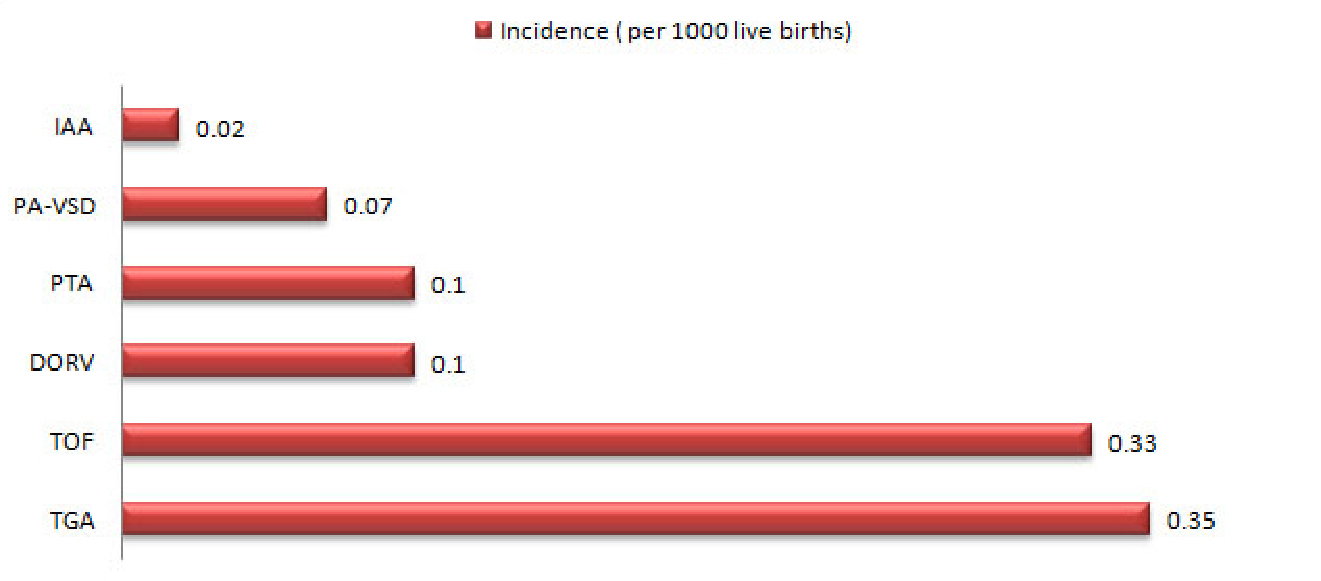
\includegraphics[scale=0.65,keepaspectratio]{Figures/Figure1_3.pdf}
\rule{35em}{0.5pt}
\caption[Incidence of different CTHDs]{Incidence of different CTHDs, per 1000 births. \cite{hoffman1995incidence}}
\label{fig:1_3}
\end{figure}

\section{Etiology}

The majority of CTHD is associated with non-cardiac malformations, and thereby constitutes syndromic forms of CTHD. These include well-known examples such as Holt-Oram syndrome, Alagille syndrome, and Noonan syndrome, among many others. Many of these syndromes have a monogenic mode of inheritance. In contrast, most non-syndromic CTHD occur sporadically, and families with a clear monogenic inheritance of non-syndromic CTHD are scarce \cite{nora1968multifactorial,emanuel1970genetics,gill2003patterns,burn1998recurrence,oyen2009recurrence}. This makes the identification of human disease genes involved in non-syndromic CTHD by a classical positional genetics approach difficult. 

Adding to the complex etiology of CTHD is the influence of exogenic factors. The environmental influences known to increase the risk of congenital heart malformations include teratogens like dioxins and pesticides \cite{kopf2009overview}, maternal alcohol consumption \cite{burd2007congenital}, smoking \cite{alverson2011maternal} and drug exposure \cite{cassina2013pregnancy,jentink2010valproic}, rubella infection during pregnancy \cite{dewan2012burden} as well as insufficient maternal folate intake \cite{ionescu2009prevalence,van2010protective}. 
Thus the sporadic nature of most non-syndromic CTHD is traditionally explained by the multifactorial inheritance model which involves a multitude of susceptibility genes with low-penetrance mutations (common variants) or high-penetrance mutations (rare variants) superposed on unfavorable environmental factors (\cref{fig:1_4}). Although widely accepted, this hypothesis remains difficult to prove, and only a handful of studies on accumulating and/or interacting effects in CTHD have been reported.

\begin{figure}[!tb]
\centering
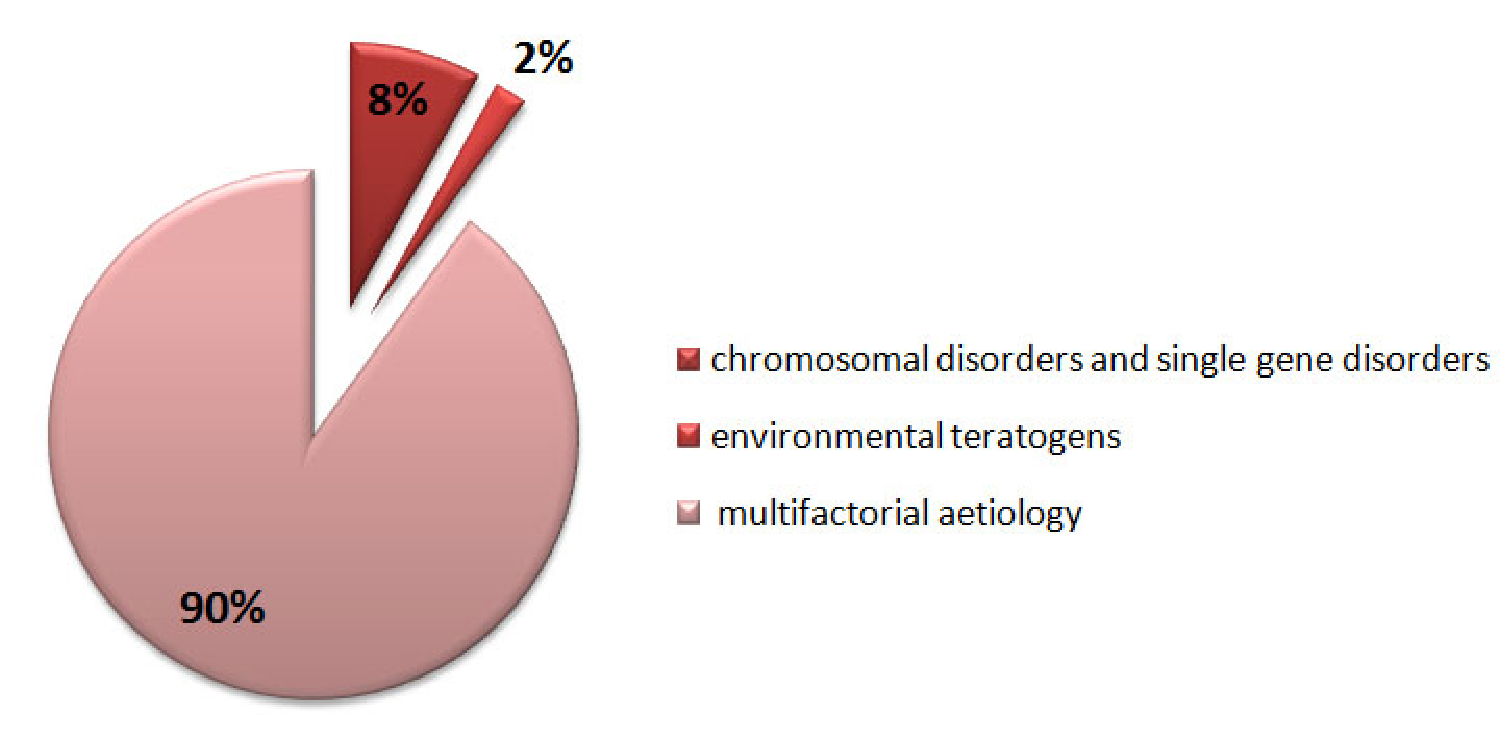
\includegraphics[scale=0.5,keepaspectratio]{Figures/Figure1_4.pdf}
\rule{35em}{0.5pt}
\caption[Etiology of CTHD]{Etiology of CTHD \cite{nora1968multifactorial}}
\label{fig:1_4}
\end{figure}

\subsection{Disease genes with high-penetrance mutations}

The fetal developmental program of the heart involves multiple pathways with extensive cross-talking and ligand–receptor interactions, secondary signal transduction pathways and a network of transcription factors that determines the expression of cardiospecific effector genes (\cref{fig:1_5}).
The majority of non-syndromic CTHD are caused by high-penetrance autosomal dominant mutations of transcriptional regulators. This includes several T-box transcription factors (\textit{TBX1}, \textit{TBX5} and \textit{TBX20}), various \textit{GATA} transcription factors (\textit{GATA4}, \textit{FOG2}), myocyte enhancer factor 2 (\textit{MEF2}), nuclear factor of activated T cells (\textit{NFAT}), serum response factor (\textit{SRF}) and homeobox transcription factors (\textit{NKX2.5}, \textit{NKX2.6}). These transcription factors also regulate the expression of numerous cardiac effector genes, including atrial natriuretic factor (\textit{ANF}), b-type natriuretic peptide (\textit{BNP}), myosins including α- myosin heavy chain  encoded by the \textit{MYH6} gene, and cardiac actin encoded by the \textit{ACTC1} gene \cite{wessels2010genetic}. Nevertheless, the majority of mutations reported in many of these genes are missense mutations of which the pathogenic, let alone the monogenic nature, has not been formally proved.

\begin{sidewaysfigure}[!p]
\centering
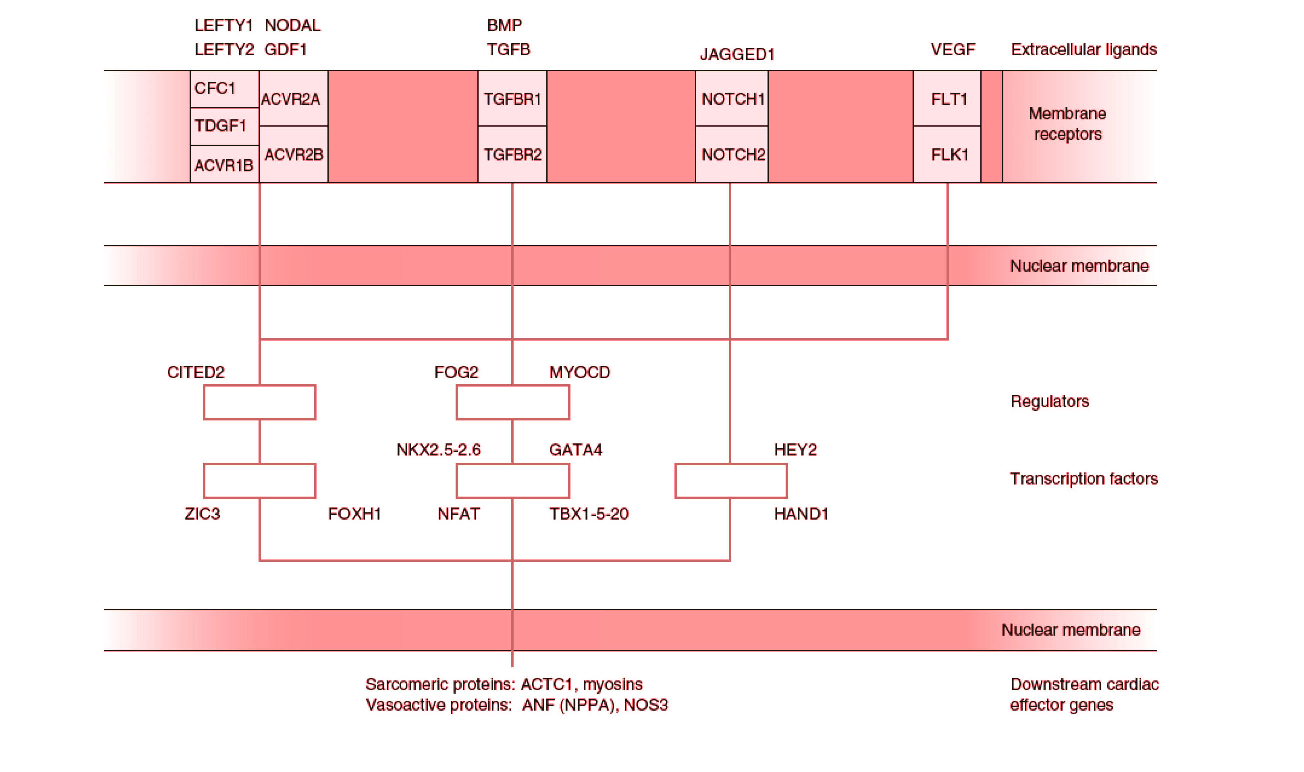
\includegraphics[scale=0.87,keepaspectratio]{Figures/Figure1_5.pdf}
\rule{35em}{0.5pt}
\caption[Signaling pathways in heart morphogenesis involved in non-syndromic CTHD]{Signaling pathways in heart morphogenesis involved in non-syndromic CTHD. The disease genes encode members of all compartments of the pathway, including ligands (\textit{LEFTY2}, \textit{NODAL}, \textit{VEGF}, \textit{GDF1}, \textit{JAGGED1}), receptors (\textit{CFC1}, \textit{TDGF1}, \textit{ACVR2B}, \textit{NOTCH1}), transcription factors-regulators (\textit{CITED2}, \textit{TFAP2B}, \textit{ZIC3}, \textit{FOXH1}, \textit{FOG2}, \textit{MYOCD}, \textit{NKX2.5-2.6}, \textit{TBX1-5-20}, \textit{GATA4}, \textit{HEY2}), and downstream effector targets including sarcomeric proteins (\textit{ACTC1}, Myosins) and vasoactive proteins (\textit{ANF}, \textit{NOS3}). Significant ligand–receptor promiscuity and cross-talking between the different signal transduction pathways exists. Source: \cite{wessels2010genetic}}
\label{fig:1_5}
\end{sidewaysfigure}

\subsection{Common variants with low-penetrance}

\begin{sloppypar} Susceptibility genes with low-penetrance mutations (common variants) are being identified rapidly for various common disorders using genome-wide association studies (GWAS). In these studies several hundred thousands of SNPs (single nucleotide polymorphisms) are analyzed simultaneously in large numbers of patients and controls using high-technology platforms. GWAS studies have not yet been performed in CTHD. However, small-scale case–control studies have identified common variants which may be associated with CTHD (\cref{tab:1_1}). As the numbers of individuals included in most of these studies are limited the conclusions are often tentative; furthermore, many studies are contradictory and have not been replicated. \end{sloppypar}

\begin{table}[!tb]
\centering
\caption[Common variants with low penetrance contributing to non-syndromic CTHD]{Common variants with low penetrance contributing to non-syndromic CTHD \cite{wessels2010genetic}}
\label{tab:1_1}

\begin{tabular}{  P{0.75in} P{0.75in} P{1.5in} P{1.5in}  }
\toprule
	\textbf{References} & \textbf{Gene}  & \textbf{Function} & \textbf{CTHD phenotypes} \\ \toprule
	\cite{christensen2009mthfd1} & \textit{MTHFD1} & Methylation cycle & TOF \\ \midrule
	\cite{van2006mtrr} & \textit{MTRR} & Methylation cycle & Various \\ \midrule
	\cite{pei2006genetic} & \textit{SLC19A1} & Methylation cycle & Various \\ \midrule
	\cite{van2008eight} & \textit{NNMT} & Methylation cycle & Various \\ \midrule
	\cite{verkleij2008genetic} & \textit{TCN2} & Methylation cycle & Various \\ \midrule
	\cite{shaw2005risks} & \textit{NPPA} & Vasoactive protein & Various \\ \midrule
	\cite{lambrechts2005low} & \textit{NOS3} & Vasoactive protein & Various \\ \midrule
	\cite{lambrechts2005low,stalmans2003vegf} & \textit{VEGF} & Polypeptide mitogen & TA, IAA, TOF \\ \midrule
	\cite{varmuza2006differential} & \textit{NFATC1} & Transcription factor & TA, IAA, TOF \\ \bottomrule
\end{tabular}
\end{table}


\subsection{Chromosomal abnormalities}

Chromosomal aberrations are also well-known causes of syndromic CTHD and are detected by conventional cytogenetics in 8–13\% of children with CTHD \cite{ferencz1989congenital}. After the introduction of fluorescence in situ hybridization (FISH) additional deletions in patients with CTHD were identified, with the 22q11.2 deletion syndrome as the prime example of a frequent cause of CTHD that escaped detection before the introduction of FISH \cite{thienpont2007submicroscopic}.

\begin{sloppypar} Newly recognized microdeletion/duplication syndromes associated with CTHD are the 22q11.1 duplication syndrome \cite{wentzel2008clinical}, the 9q34 deletion syndrome \cite{stewart2007chromosome}, the 17p11.2 deletion syndrome \cite{andrieux2007genotype}, the 16p11.2 deletion syndrome \cite{brunetti2008recurrent,hernando2002comparative} and the 1q21.1 deletion syndrome \cite{brunetti2008recurrent,mefford2008recurrent,christiansen2004chromosome}. These microdeletions/ duplications are good candidate regions to identify CTHD genes. Some of the known microdeletion syndromes, such as the 22q11.2 deletion syndrome, can present with CTHD without obvious dysmorphic features and/or mental deficit. The recently recognized 1q21.1 microdeletion or -duplication syndrome has an even more variable phenotype with incomplete penetrance \cite{brunetti2008recurrent,mefford2008recurrent,christiansen2004chromosome}. In a large series of 1q21.1 deletion patients, 25\% presented with CTHD \cite{mefford2008recurrent}. This deletion was also found in 3 out of 505 patients with non-syndromic CTHD \cite{christiansen2004chromosome}. Overall, a high frequency of chromosomal deletions, duplications and copy number variations (CNV) was recently found in two series of non-syndromic patients with CTHD \cite{erdogan2008high,greenway2009novo}. These studies also indicated that array comparative genomic hybridization could be a powerful tool to identify new loci involved in non-syndromic CTHD, and furthermore a useful tool in the diagnostic workup of patients with non-syndromic CTHD. \end{sloppypar}
 
\subsection{Somatic mutations}

Knudson has elegantly shown how somatic mutations not present in the germline can contribute to genetic disease with his two-hit hypothesis \cite{knudson1972mutation}. These somatic mutations not only include mutations affecting nuclear DNA leading to activation of oncogenes or inactivation of tumor suppressor genes, but also epigenetic alterations of DNA, and mitochondrial DNA mutations. Surprisingly, many years after Knudson’s theory gained universal acceptance, the concept of somatic mutations remained largely confined to tumor biology and skin disease. This might explain why the candidate gene approach for many non-syndromic malformations, including CTHD, has had little success. Mutation analysis in most cases still is usually performed in constitutional DNA, whereas the mutations might be somatic and limited to the affected tissue. Over the last past years, the first somatic mutations confined to affected cardiovascular tissue have been reported in CTHD. 
The group of Reamon-Buettner and Borlak \cite{reamon2006bridging,reamon2006hey2,reamon2004tbx5,reamon2004novel,reamon2004somatic,reamon2006somatic,reamon2008loss} has reported the majority of somatic mutations in CHD, including mutations in \textit{NKX2.5}, \textit{TBX5}, \textit{GATA4}, \textit{HEY2} and \textit{HAND1}.

Interestingly, in several patients’ different mutations in the same gene with cumulative down regulation of transcription was reported \cite{reamon2006bridging,reamon2006hey2,reamon2004tbx5,reamon2004novel,reamon2004somatic,reamon2006somatic,reamon2008loss}. Only a limited number of studies have been performed, most probably due to the scarceness of affected cardiac tissue. Recently, no evidence for somatic \textit{NKX2.5} mutations was found in a series of fresh-frozen cardiac tissue taken near the septal defect of patients with ASD, VSD and AVSD \cite{draus2009investigation}. The latter authors suggested that the poor DNA quality from the formalin-fixed tissue used by the group of Reamon-Buettner and Borlak may account for the high amount of somatic mutations in their study, although differences in the location of tissue sampling might also be important. Evidently, the role of somatic mutations in CTHD awaits further confirmation.

Despite all these huge advances that have been made in understanding the etiology of congenital heart malformations, the underlying causes for a majority of CTHD still remain unclear. Given the spatiotemporal complexity of cellular differentiation pathways in the developing heart, it seems conceivable that a large number of intercellular signalling modules and intracellular transcriptional circuits act together to achieve cardiac regionalization. Although the complexity of these molecular players and their interactions in CTHD are not yet completely understood, a wealth of information suggests that three specific metabolic and developmental pathways could contribute to the etiology; which includes the transcription factor \textit{TBX1}, the molecular marker of the cardiac lineage \textit{NKX2.5} and variants of the folate-homocysteine metabolic axis.

\section{\textit{TBX1} and SHF development}


Members of the T-box gene family are important regulators of myocardial proliferation and patterning. The \textit{TBX} subfamily consists of many molecular players like \textit{TBX1}, \textit{TBX18} and \textit{TBX20}; similarly, the \textit{TBX2} subfamily, \textit{TBX2}, \textit{TBX3} and \textit{TBX5} and have all been found to play specific roles in heart development \cite{naiche2005t,plageman2005t,stennard2005t,merscher2001tbx1}. T-box genes encode transcription factors that are characterized by a highly conserved DNA-binding region which recognizes a specific DNA element, the T-half site, that occurs singly, or in multiples with different orientation and spacing in promoters of target genes, and mediates transcriptional activation and/or repression. \cref{tab:1_2} summarizes the role of T-box genes in heart development.

\textit{TBX1} is required in the pharyngeal mesoderm \cite{naiche2005t} and for a reservoir of cardiac progenitor cells that gradually migrate and populate the OFT, RV, and parts of the atria. Genetic lineage studies have demonstrated that \textit{TBX1}-positive cells in the SHF provide extensive contributions between embryonic day (E) 8.5 and E9.5 to the outflow tract

\begin{landscape}
\begin{table}[!p]
\renewcommand{\arraystretch}{1.4}
\centering
\caption[T-box transcription factors]{T-box transcription factors and their roles in regulatory hierarchies in the developing heart \cite{stennard2005t}}
\label{tab:1_2}
\begin{tabular}{  P{1in} P{1in} p{4.5in}  P{2in}  }
\toprule
	\textbf{Gene} & \textbf{Chromosome} & \textbf{Main expression sites during embryogenesis} & \textbf{Associated human disease} \\ \toprule
	\textit{TBX1} & 22q11.21 & pharyngeal endoderm, mesodermal core of first pharyngeal arch;  endoderm lining posterior pharyngeal pouches, head mesoderm ventral to hindbrain including secondary heart lineage mesoderm, sclerotome & 22q11 microdeletion syndrome \\ \midrule
	\textit{TBX2} & 17q23.2 & allantois; non-chamber myocardium; optic and otic vesicles, naso-facial mesenchyme, limbs, lungs, genitalia & None identified. \\ \midrule
	\textit{TBX3} & 12q24.21 & non-chamber myocardium, specifically sinuatrial region, AV canal and interventricular ring; eventually delineates the cardiac central conduction system & Ulnar mammary syndrome \\ \midrule
	\textit{TBX4} & 17q21-q22 & Hindlimb, proctodeum, mandibular and lung mesenchyme, atrium and body wall & Small patella syndrome \\ \midrule
	\textit{TBX5} & 12q24.1 & Cardiac crescent, heart tube (graded, highest caudally), sinus venosus, common atrium, LV, trabeculae of the RV, forelimb, eye & Holt Oram syndrome \\ \midrule
	\textit{TBX18} & 6q14.1-q15 & Splanchnic mesoderm, septum transversum, proepicardial organ, epicardium & None identified. \\ \midrule
	\textit{TBX20} & 7p14.3 & Allantois, lateral plate mesoderm, cardiac crescent, heart, endocardial cushions & None identified. \\ \bottomrule
\end{tabular}
\end{table}
\end{landscape}

 myocardium, endocardium and mesenchymal cushions \cite{naiche2005t,plageman2005t}, suggesting that \textit{TBX1} is expressed in the larger SHF. \textit{TBX1} cell-autonomously maintains the cardiac progenitor population within the SHF by enhancing cell proliferation and inhibiting cardiomyocyte differentiation.

Tracing of the \textit{TBX1}-positive lineage revealed that in a \textit{TBX1}-deficient background there was reduced cell proliferation, which may underlie the reduced contribution of the SHF to the OFT \cite{naiche2005t,plageman2005t,stennard2005t}. Furthermore, mice that were \textit{Tbx1} haplosufficient phenocopied important aspects of the 22q11 microdeletion syndrome, including OFT abnormalities. This demonstrates its specific function in the developing mammalian heart \cite{merscher2001tbx1,jerome2001digeorge,liao2004full}.


T-box genes, however, are not only conserved DNA-binding regions, but also conserved interaction domains for other transcription factors. A synergistic interaction between \textit{TBX1} and \textit{NKX2.5} has recently postulated to play a role in the 22q11 microdeletion syndrome \cite{nowotschin2006tbx1}.

It has been hypothesized that \textit{NKX2.5} acts as a T-box guidance factor instead of a direct transcriptional activator or repressor. Moreover, \textit{TBX1} binds to a critical \textit{PITX2} enhancer and synergistically together with \textit{NKX2.5} induces transcriptional activity of this enhancer. This further indicates that \textit{TBX1} and \textit{NKX2.5} act in the same pathway for outflow tract morphogenesis, making it the next obvious candidate gene for CTHD.

\subsection{\textit{NKX2.5} as a central regulator of heart development}

The homeodomain protein \textit{NKX2.5} controls many aspects of cardiac development, beginning with specification and proliferation of cardiac precursors to later events, such as the formation of the outflow tract \cite{harvey2002patterning}. \textit{NKX2.5} acts near the top of a large transcriptional cascade controlling multiple cardiac genes, with its expression regulated by \textit{GATA} factors and \textit{SMAD} proteins and by \textit{NKX2.5} itself in an auto-regulatory loop \cite{liberatore2002nkx,lien2002cardiac,lien1999control,searcy1998gata}. More recently, \textit{NKX2.5} expression in the second heart field was shown to be dependent on the \textit{ISL1}, while interactions between \textit{NKX2.5}, \textit{BMP2}, and \textit{SMAD1} control cardiac progenitor specification and proliferation \cite{prall2007nkx2,takeuchi2005tbx20}.

\textit{NKX2.5} acts in combination with other core cardiac transcription factors to promote cardiomyocyte differentiation and chamber identity. For example, \textit{NKX2.5} and the basic helix-loop-helix protein \textit{HAND2} cooperate to activate \textit{IRX4}, which is necessary for determining ventricular identity \cite{yamagishi2001combinatorial}. Ventricular identity is also controlled by \textit{NKX2.5} through a direct physical interaction with the \textit{MADS} box transcription factor \textit{MEF2C} \cite{vincentz2008cooperative}. In addition, \textit{NKX2.5} interacts with another \textit{MADS} box transcription factor, \textit{SRF}, and \textit{GATA4} to promote cardiac sarcomeric protein gene expression \cite{sepulveda2002combinatorial}. \textit{NKX2.5} also plays a role in outflow tract development through regulation of the transcriptional repressor \textit{JARID2} \cite{barth2010jarid2}.

In mice, loss of \textit{NKX2.5} results in embryonic lethality with failure of cardiac looping and deficient myocardial differentiation \cite{lyons1995myogenic,tanaka1999cardiac}. \textit{NKX2.5} heterozygous mice have progressive atrioventricular (AV) block, a phenotype similar to part of the spectrum of congenital heart disease phenotypes described in human patients with \textit{NKX2.5} mutations \cite{benson2010genetic,biben2000cardiac}. In addition, mutation of \textit{SHOX2}, an upstream transcriptional repressor of \textit{NKX2.5} expressed in the sinoatrial node (SAN), results in mid-gestational embryonic lethality in mice with severe hypoplasia of the SAN and associated abnormal heart rate \cite{blaschke2007targeted,espinoza2009shox2}. Consistent with these observations, mutations in \textit{NKX2.5} have been found in patients with a variety of structural malformations including septation defects, alignment defects, and compaction defects, and cardiac conduction defects \cite{reamon2010nkx2,jay2004nkx2}. Thus, the essential role of \textit{NKX2.5} in multiple distinct aspects of heart development and congenital heart disease suggests that mutations in this early molecular marker of the cardiac lineage are likely to be associated with CTHD \cite{moskowitz2007molecular}.

\subsection{Variants of the folate-homocysteine metabolic axis}

Advances in surgical techniques and in utero diagnosis promoting delivery in specialized centers have considerably improved the prospects for children born with CTHD and made a tremendous impact on mortality. However, the surgeries needed to correct many of the anatomical defects can greatly compromise the quality of life. Therefore, preventing CTHD is still a major goal and identification of pathways that could be manipulated by micronutrients to prevent CTHD is one step towards this aim.

The first studies showing that vitamin B might be involved in the pathogenesis of congenital anomalies originate from the 1950s. Multiple congenital malformations including cardiovascular defects were observed in rats when a folic acid deficient diet was given to female rats in early pregnancy \cite{nelson1952production,baird1954congenital}. Some decades later, the role of vitamin B in vascular pregnancy complications was reported. Mothers of a child with a congenital malformation and women with placental abruption showed a folate deficiency \cite{hibbard1965folic,smithells1976vitamin}. Also, maternal hyper-homocysteinaemia has been associated with a three-to-tenfold increased risk of CHD \cite{kirby1983neural,bartelings1985contribution,shaw1995maternal}. It was suggested that homocysteine affects cardiac neural crest cell behavior thereby leading to the development of cardiac malformations \cite{boot2003folic}. Interestingly, folic acid supplementation partially rescues these detrimental effects of homocysteine on neural crest cell outgrowth. Thereafter, several epidemiological studies reported that the use of folic acid containing supplements in the periconceptional period reduced the risk of having a child with a CHD \cite{botto1996periconceptional,czeizel1998periconceptional,botto2000occurrence}.

\begin{sloppypar} Folic acid (FA) is central to folate-requiring one-carbon metabolism, which play key roles in numerous cellular reactions. These involve amino acid metabolism, biosynthesis of purine and pyrimidine, and formation of primary methylating agent S-adenosyl-methionine (SAM), which is the universal methyl donor for DNA, histones, proteins and lipids \cite{boot2004cardiac}. Mechanistically, the transport of transmembrane folate is facilitated by both receptors and specific carriers active across cell membranes \cite{fowler2001folate}. Under normal circumstances, natural dietary folate is absorbed in the intestine and/or liver and metabolized primarily to 5-methyl tetrahydrofolate (5-methylTHF) and subsequently gets polyglutamated for cellular retention However, FA consumed in fortified foods/supplements is reduced primarily to dihydrofolate by the enzyme dihydrofolate reductase in the liver and finally converted to the tetrahydrofolate (THF), the substrate for polyglutamate synthetase. The polyglutamyl form of THF formed either from FA or normal dietary folate is the central folate acceptor molecule in the one-carbon cycle. Next, THF is converted to 5,10-methyleneTHF by vitamin B6 dependent serine hydroxymethyltransferase and then reduced irreversibly to 5-methylTHF by methylenetetrahydrofolate reductase (MTHFR). 5-Methyl-THF acts as a primary methyl donor for the remethylation of homocysteine to methionine. Methonine is a key substrate for S-adenosylmethionine (SAM) which plays a central role in methylation reactions catalyzed by DNA methyltransferases (DNMTs) forming 5-methylcytosine \cite{stanger2002physiology,crider2012folate,hubner2009folate,liu20104,zhang2013genetic}. Thus, the entire FA metabolism is modulated by several folate coenzymes. Mechanistically, the central role of these coenzymes is to modulate the metabolic pathway by accepting or donating one-carbon units. \end{sloppypar}

The link between low folate/high homocysteine and heart defect incidence implies that SNP in the folate pathways may be genetic risk factors for congenital malformations like CTHD. Key genes in this pathway that are involved in transferring the methyl group to homocysteine, and have been most extensively studied include methylenetetrahydrofolate reductase (\textit{MTHFR}), methionine synthase reductase (\textit{MTRR}), reduced folate carrier (\textit{RFC}), along with vitamin B12- dependent methionine synthase (\textit{MTR}) \cite{zhang2013genetic} (\cref{fig:1_6}). Polymorphisms in these folate pathway genes appear to affect protein function and/or folate metabolism and thus may affect the risk for heart defects. 

\begin{figure}[!tb]
\centering
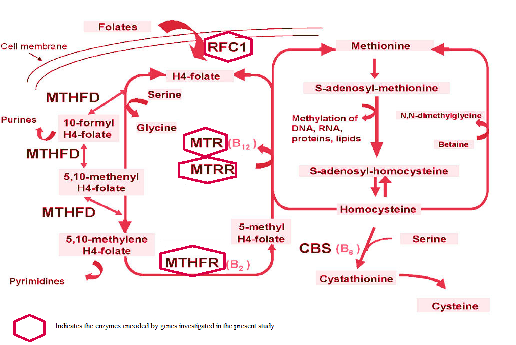
\includegraphics[scale=1.5,keepaspectratio]{Figures/Figure1_6.pdf}
\rule{35em}{0.5pt}
\caption[Overview of the homocysteine and folate metabolic pathway]{Overview of the homocysteine and folate metabolic pathway. Source: \cite{fowler2001folate}}
\label{fig:1_6}
\end{figure}

The mother is the environment of the developing child in utero and, therefore, the maternal nutritional status will influence the homocysteine metabolism in the embryonic tissues as well. Expression of functional polymorphisms in vitamin B related genes derived from both parents might also be important in the development of the embryonic heart. In addition, interactions should be considered between the maternal nutritional status and the polymorphisms in vitamin B related genes of mothers and children. 

\section{Justification for the research study}

Over the past decade investigators have witnessed remarkable advances in our understanding of cardiogenesis, and the heart has become one of the well-understood organs in biology. This knowledge is now being used to discover the underlying genetics of CHD and the basis for many adult-onset diseases that have their origin in mutations of developmental genes. What is lacking is a coherent picture of the hierarchical pathways that govern most developmental processes and the mechanisms through which such pathways regulate the cell biology of morphogenesis. Such knowledge will require a better understanding of the target genes of critical transcriptional and signaling pathways that control cardiogenesis. 

Research in this area will be an essential step, as the targets will be the most amenable sites of intervention, both in a therapeutic sense and for the purpose of prevention. For example, identification of dietary substances that modulate key developmental pathways such as folic acid, which prevents neural tube defects, will be necessary for preventive efforts. In addition, early genetic identification of those at risk for adult-onset disease originating from a cardiac developmental defect will provide ample time for intervention to slow the progression of disease. Based on the premise that the simultaneous assessment of multiple factors would aid in identifying genetic causative and risk factors in CTHD, the hypothesis, aim and objectives of this thesis was formulated.

\section{Hypothesis}

A combination of a haploinsufficiency of \textit{TBX1}, rare mutations in \textit{NKX2.5} and folate-related SNP may contribute to the risk of developing CTHD and define its polygenic origin.

\section{Aim}

The aim of the study is to identify association of mutations or variations in selected candidate genes (T‐box transcription factor \textit{TBX1}, earliest molecular marker of the cardiac lineage \textit{NKX2.5} and genes of the folate-homocysteine metabolic axis) with CTHD. 

\section{Objectives}

\begin{sloppypar}
\begin{enumerate}
\item To screen for chromosomes abnormalities, in particular 22q11.2 microdeletion, in the blood lymphocytes of children with CTHD.
\item To determine the frequency of sequence variants in T box transcription factor \textit{TBX1} in cases with non-syndromic CTHD. 
\item To identify the spectrum of cardiac transcription factor \textit{NKX2.5} mutations and sequence variants and then relate it to CTHD.
\item To identify common polymorphisms in rs1801133, rs1801131 of \textit{MTHFR}, rs1051266 of \textit{SLC19A1}, rs1805087 of \textit{MTR}, rs1801394 and rs1532268 of \textit{MTRR} involved in folate metabolism and its association with CTHD.
\end{enumerate}
\end{sloppypar}

\clearpage
\printbibliography[heading=subbibintoc]
\end{refsection}

